% =====================================================================
%  IJIST (Wiley) submission -- built on the official Wiley NJD template
%  (USG.cls v6.0, 2024-05-07), downloaded by the author and placed in
%  template/. See template/Author-guidelines for LaTex Template_Wiley
%  (2026).pdf for the template's own instructions.
%
%  Reference style: numbered (VANCOUVER option), matching main_updated.tex's
%  existing numbered citations and IJIST's own published-article convention
%  (the checklist notes the stated APA style is nominal; numbered references
%  are accepted under Free Format). No .bst for VANCOUVER ships in the
%  downloaded template bundle (only wileyNJD-Chicago.bst), and this
%  environment has no LaTeX engine to test bibtex anyway, so the
%  bibliography is an inline \thebibliography block (manually numbered),
%  the same mechanism paper/main_updated.tex already used successfully --
%  no bibtex run required at all.
%
%  STATUS: assembled from the approved section drafts in Wiley-IJIST.md
%  (Title/Abstract/Keywords, Introduction, Materials and Methods, Results,
%  Discussion, Conclusion -- all approved 2026-11-06). This file has NOT
%  been compiled in this environment (no local LaTeX engine available).
%  Compile via Overleaf or a local TeX distribution and report any errors
%  back for fixing -- see Wiley-IJIST.md's decision log for this call.
%
%  OPEN ITEMS carried into this file as TODO/VERIFY comments -- search for
%  "VERIFY" below. None of these block compilation; they block submission.
% =====================================================================

\documentclass[VANCOUVER,twocolumn]{USG}
\usepackage{anyfontsize}
\usepackage{colortbl}
\usepackage{xcolor}
\usepackage{amsmath,amssymb,amsfonts}
\usepackage{graphicx}
\usepackage{booktabs}

\graphicspath{{./figures/}}

\articletype{ORIGINAL ARTICLE}

% VERIFY: received/revised/accepted dates, volume, copyyear, article DOI --
% all assigned by the journal at submission/acceptance; placeholders only.
%\received{}
%\revised{}
%\accepted{}
\journal{International Journal of Imaging Systems and Technology}
\volume{0}
\copyyear{2026}
\startpage{1}
%\articledoi{10.1002/ima.XXXXX}

\begin{document}

\title{A Calibrated Soft-Voting Ensemble for Skin Disease Classification in Melanin-Rich Skin}
\titlemark{Calibrated Ensemble for Melanin-Rich Skin}
% running title above is 38 characters, within IJIST's 40-character limit

% ---------------------------------------------------------------------
% VERIFY: author order, affiliations, and ORCID iDs are carried over
% unchanged from paper/main_updated.tex. ORCID placeholders below are
% empty per-author -- the user must supply each iD (at minimum the
% corresponding author's, per IJIST's stated requirement) before
% submission.
%
% FIX (2026-11-07, first Overleaf compile error): USG.cls does NOT define
% a starred \author* (that is Springer sn-jnl's convention, not Wiley
% NJD's), and \fnm{}/\sur{} are not meant to be nested inside \author{} as
% the display name -- USG.cls's own working example
% (template/Optimal-Design-layout.tex) uses plain \author[N]{Full Name}.
% Using \author*[5]{\fnm{Neha}\sur{Katre}} broke argument parsing and left
% \sur undefined. Corresponding-author status is conveyed entirely by the
% separate \corres{} macro below (confirmed against the working example),
% not by starring \author. \address{} also does not accept a comma-list of
% affiliation numbers ([1,2,3,4,5]) -- USG.cls's \@@address takes exactly
% one optional numeric argument, so one \address[N]{} call per author
% number is required, matching the example exactly (repeating the same
% affiliation text, since all five authors share one).
% ---------------------------------------------------------------------
\author[1]{Manav Jain}
\author[2]{Dhruv Bhagchandani}
\author[3]{Mohammed Ali Fatteh}
\author[4]{Rohan Dhand}
\author[5]{Neha Katre}
% VERIFY: confirm Neha Katre is intended as the IJIST corresponding
% author (she is the one given an email/\corres{} entry below, carried
% over from main_updated.tex's \author* marking).

\address[1]{\orgdiv{Information Technology}, \orgname{Dwarkadas J. Sanghvi College of Engineering}, \orgaddress{\street{Bhaktivedanta Swami Marg, Vile Parle (W)}, \city{Mumbai}, \postcode{400056}, \state{Maharashtra}, \country{India}}}
\address[2]{\orgdiv{Information Technology}, \orgname{Dwarkadas J. Sanghvi College of Engineering}, \orgaddress{\street{Bhaktivedanta Swami Marg, Vile Parle (W)}, \city{Mumbai}, \postcode{400056}, \state{Maharashtra}, \country{India}}}
\address[3]{\orgdiv{Information Technology}, \orgname{Dwarkadas J. Sanghvi College of Engineering}, \orgaddress{\street{Bhaktivedanta Swami Marg, Vile Parle (W)}, \city{Mumbai}, \postcode{400056}, \state{Maharashtra}, \country{India}}}
\address[4]{\orgdiv{Information Technology}, \orgname{Dwarkadas J. Sanghvi College of Engineering}, \orgaddress{\street{Bhaktivedanta Swami Marg, Vile Parle (W)}, \city{Mumbai}, \postcode{400056}, \state{Maharashtra}, \country{India}}}
\address[5]{\orgdiv{Information Technology}, \orgname{Dwarkadas J. Sanghvi College of Engineering}, \orgaddress{\street{Bhaktivedanta Swami Marg, Vile Parle (W)}, \city{Mumbai}, \postcode{400056}, \state{Maharashtra}, \country{India}}}

\corres{Neha Katre (\email{neha.medjoge@djsce.ac.in})}
% VERIFY: full postal address for the corresponding author -- IJIST
% requires this; only the email is carried over from main_updated.tex.

\fundingInfo{VERIFY: funding source(s) and grant/award number(s), or
state ``This research received no specific grant from any funding
agency.'' -- user to supply, see Wiley-IJIST.md Phase 8.}

\keywords{skin disease classification | deep learning ensemble | model calibration | ConvNeXt | Swin Transformer | melanin-rich skin | Fitzpatrick skin type}

\abstract[ABSTRACT]{Computer-aided diagnostic tools for skin disease often
perform less well on melanin-rich skin, both because training data are
dominated by lighter Fitzpatrick skin types and because pigmentation can
mask the erythema that many visual diagnostic criteria depend on. Ensemble
classifiers proposed for dermatological screening are usually justified on
accuracy alone, without examining whether their probability estimates are
calibrated -- a property that determines whether a ranked differential
diagnosis can be trusted. We curate a five-class corpus of 6,655 images
(basal cell carcinoma, eczema, keratosis, melanoma, and tinea) from five
public sources and audit it for cross-split near-duplicates using
perceptual hashing, which identifies and removes 162 contaminated test
images (22.3\%). On the resulting de-duplicated 565-image test set, we
evaluate three ImageNet-pretrained backbones (EfficientNet-B1, Swin-Tiny,
and ConvNeXt-Tiny) individually and in every combination. The most accurate
single backbone, ConvNeXt-Tiny (88.67\% accuracy), is also the
worst-calibrated and most overconfident of the three (expected calibration
error [ECE] 0.0497). We propose an equal-weight soft-voting ensemble of all
three backbones; no weight search was performed on any split. The ensemble
attains 87.79\% accuracy (95\% CI 84.96--90.44\%) and a macro-averaged area
under the receiver operating characteristic curve (AUC) of 0.9813 (95\% CI
0.9744--0.9872), significantly exceeding every individual backbone and
every two-backbone subset on macro-AUC (paired bootstrap, all 95\% CIs
excluding zero). The ensemble's calibration error (0.0352) is lower than
ConvNeXt-Tiny's and is the only configuration with slightly conservative
rather than overconfident mean confidence; temperature scaling fitted on
validation reduces test ECE further to 0.0216 without changing any
prediction. Sensitivity reaches 100.00\% for basal cell carcinoma and
97.58\% for melanoma. Skin-tone labels are not consistently available
across the five sources, so tone-stratified performance is not reported.
Ensembles intended for skin-disease screening should be selected and
reported on calibration as well as accuracy.}

% ---------------------------------------------------------------------
% Key points (optional, <=3 per the checklist)
% ---------------------------------------------------------------------
\begin{itemize}
\item The most accurate single backbone (ConvNeXt-Tiny, 88.67\% accuracy) is also the worst-calibrated and most overconfident of the three.
\item A three-backbone soft-voting ensemble improves ranking quality (macro-AUC 0.9813, significantly above every single backbone and every two-backbone subset) and is the only configuration with slightly conservative rather than overconfident probabilities.
\item The ensemble retains 100\% basal cell carcinoma and 97.58\% melanoma sensitivity on a de-duplicated, 565-image melanin-rich test set.
\end{itemize}

\maketitle

% =======================================================================
\section{Introduction}\label{sec:intro}
% =======================================================================

Dermatological disorders are a major health burden worldwide, ranging from
non-cancerous inflammatory conditions to malignant melanomas, and early,
accurate diagnosis is central to effective treatment.
% VERIFY (Phase 7, 2026-11-06): this opening claim currently carries no
% citation. ref1 (Aboulmira et al., a methods survey of ML/DL skin-disease
% classification techniques) was checked and does not support a
% clinical-outcomes claim -- it surveys classification methods, not
% treatment effectiveness or mortality. Either find a genuine
% clinical-outcomes source or accept this as an uncited general premise.
In South Asia, fungal infections, pigmentation disorders, and eczematous
dermatoses are highly prevalent, and diagnosis is frequently delayed, which
worsens patient outcomes and strains local healthcare infrastructure.

A key obstacle to both clinical and algorithmic diagnosis in this
population is melanin concentration. Skin diseases present differently in
melanin-rich skin than in lighter skin: erythema, the sign on which many
visual diagnostic criteria depend, may be masked or may appear instead as
hyperpigmentation.
% VERIFY: this clinical fact currently carries no citation -- needs a
% dermatology textbook/review source, not yet in references.bib.
Computer-aided diagnostic (CAD) systems developed largely from
lighter-skinned clinical atlases often do not transfer well to melanin-rich
presentations: skin-lesion segmentation networks show systematically lower
performance on darker Fitzpatrick types, and common mitigation strategies
do not fully close the gap \cite{ref6}; a large multimodal language model
similarly showed significantly lower diagnostic sensitivity, specificity,
and accuracy for melanoma in Fitzpatrick types III--VI than in types I--II
\cite{ref10}. These failures disproportionately disadvantage affected
populations and contribute to disparities in care.

Representation at scale has not resolved this gap. A dermatology
foundation model pretrained on more than two million images improved
results across twenty-eight benchmarks \cite{ref2}, indicating that the
limiting factor is what the training images represent rather than how the
model is built. Several recent corpora address this directly by collecting
melanin-rich and region-specific imagery rather than augmenting existing
Western archives \cite{ref3,ref4,ref5}, and audits of skin-lesion models
have found systematically lower performance on darker skin types that
common mitigation strategies do not fully close \cite{ref6}.

Ensemble learning is a natural response to the resulting data and model
uncertainty: combining heterogeneous architectures can increase robustness
and predictive accuracy beyond what any single network achieves
\cite{ref14,ref15}. However, ensembles for dermatological screening are
typically evaluated and justified on accuracy and area under the receiver
operating characteristic curve (AUC) alone. A classifier that is
confidently wrong can suppress a referral that an appropriately uncertain
one would prompt, so whether an ensemble's probability estimates are
calibrated is at least as clinically relevant as its accuracy. To our
knowledge, the calibration of heterogeneous convolutional-transformer
soft-voting ensembles has not been examined on a melanin-rich clinical
corpus.
% VERIFY: this "to our knowledge" novelty claim needs checking against the
% cited ensemble papers' own reported metrics (ref12-ref17) before
% finalizing, per the governing prompt's own instruction -- not yet done,
% requires reading each paper's results section.

This study addresses that gap. The intended use is decision support for
dermatologists: the system returns a ranked probability vector for
clinician review and is not designed to diagnose autonomously. We make
three contributions. First, we curate a five-class corpus of 6,655 images
from five public sources and audit it for cross-split near-duplicates
using perceptual hashing, removing contaminated test images before
reporting any result. Second, we evaluate all seven combinations of three
backbones -- EfficientNet-B1, Swin-Tiny, and ConvNeXt-Tiny -- on accuracy,
macro-AUC, the Matthews correlation coefficient, and expected calibration
error, and show that the most accurate configuration is also the worst
calibrated. Third, we propose an equal-weight three-backbone soft-voting
ensemble that retains the sensitivity needed for malignant classes while
producing better-calibrated, slightly conservative probabilities instead
of overconfident ones.

% =======================================================================
\section{Materials and Methods}\label{sec:methods}
% =======================================================================

\subsection{System Overview}

The classification engine evaluated in this study is one component of a
larger clinically integrated pipeline: image acquisition and quality
checking, preprocessing, the ensemble classifier, an explainability layer,
and a deterministic severity-triage module that applies clinical safety
overrides before an LLM-based summary is generated. This study evaluates
only the image classification engine (preprocessing and ensemble model);
clinical decision-support modules (treatment recommendations, specialist
referral, and user authentication) are specified as design goals and are
not yet implemented, and metadata integration (patient age, sex, medical
history) is a deployment-path feature not exercised in the present
evaluation, since the aggregated public corpora used here do not carry a
consistent metadata schema.

\subsection{Datasets}

A five-class corpus of 6,655 images was assembled from five public
sources: Fitzpatrick17k, PAD-UFES-20, DermaCon-IN \cite{ref5}, the Melanoma
Cancer Image Dataset, and the Skin Disease Image Dataset (SDID).
% VERIFY: Fitzpatrick17k, PAD-UFES-20, Melanoma Cancer Image Dataset, and
% SDID have no bibliography entry yet -- see references.bib comments and
% Wiley-IJIST.md Phase 7 \S2.2 for draft entries (two drafted, two still
% unidentified).
The five classes retained from a larger nine-class pool (which additionally
contains acne, lichen planus, psoriasis, and vitiligo) are basal cell
carcinoma, eczema, keratosis, melanoma, and tinea, selected as the
conditions most relevant to a screening task. Table~\ref{tab:dataset} gives
the per-class distribution.

\begin{table}[htbp]
\caption{Class-wise distribution of the curated dataset.}\label{tab:dataset}
\begin{tabular}{@{}lrrrr@{}}
\toprule
Disease Class & Train & Val & Test & Total \\
\midrule
Basal Cell Carcinoma & 968 & 119 & 121 & 1,208 \\
Eczema & 1,072 & 148 & 145 & 1,365 \\
Keratosis & 977 & 159 & 158 & 1,294 \\
Melanoma & 1,197 & 202 & 188 & 1,587 \\
Tinea & 966 & 120 & 115 & 1,201 \\
\midrule
Total & 5,180 & 748 & 727 & 6,655 \\
\botrule
\end{tabular}
\end{table}

The corpus was partitioned into training, validation, and test subsets in
an approximate 78:11:11 ratio (5,180/748/727 images). This partition was
inherited as a fixed folder structure rather than generated by code
available for inspection in this study; the per-class proportions in
Table~\ref{tab:dataset} are consistent with stratification by disease
class, but we did not independently verify the partitioning procedure
itself, and no patient- or lesion-level identifiers are available across
the five aggregated sources to confirm that no patient appears in more
than one partition.

A post-hoc perceptual-hash audit (Hamming distance $\leq$ 5) identified 162
test images (22.3\%) with a near-duplicate in the training or validation
partitions. All test-set metrics reported in this paper are computed on
the resulting de-duplicated 565-image subset (106 basal cell carcinoma,
111 eczema, 133 keratosis, 124 melanoma, 91 tinea) unless otherwise stated;
we did not similarly screen the training and validation sets for internal
duplication, which would affect training signal rather than measurement
validity.

The corpus is mildly imbalanced: the largest class (melanoma, 1,197
training images) exceeds the smallest (tinea, 966) by a ratio of
approximately 1.24 to 1.

\subsection{Model Architecture}

The classification engine is a soft-voting ensemble of three independently
fine-tuned backbones, each accepting a $224\times224\times3$ input and
producing its own five-class probability distribution: EfficientNet-B1,
which uses mobile inverted-bottleneck convolution blocks with
squeeze-and-excitation channel attention to capture fine-grained texture
\cite{ref27}; Swin-Tiny, which uses shifted-window self-attention to
capture long-range spatial dependencies \cite{ref11}; and ConvNeXt-Tiny,
which uses large-kernel depthwise convolution with Layer Normalization to
combine convolutional and transformer design principles \cite{ref12}. Each
backbone's pooled feature vector ($1280$-d for EfficientNet-B1, $768$-d for
the other two) feeds an independent classification head (Layer
Normalization, a two-layer MLP with GELU activations, dropout 0.35 for
EfficientNet-B1 and 0.4 for the other two). The three branches are trained
independently; no fusion network, learned projection, or shared head
exists. Full per-layer equations for each backbone are given in Supporting
Information S1.

The ensemble prediction is the equal-weight average of the three softmax
outputs,
\begin{equation}
p_k = \frac{1}{3}\sum_{b \in \{\mathrm{eff,swin,conv}\}} p_{b,k}
\end{equation}
No weight search was performed on any split; equal weighting was retained
as a deliberate design choice to avoid overfitting the combination rule to
a held-out set. An agreement score -- the fraction of backbones whose
individual top-1 prediction matches the ensemble's -- is produced alongside
the prediction as a confidence signal.

\subsection{Training Configuration}

Each backbone was initialized from ImageNet-pretrained weights and
fine-tuned independently with its own hyperparameters
(Table~\ref{tab:hyperparams}), since the three architectures differ
substantially in depth and parameter count. All three used AdamW
\cite{ref26} with a two-phase schedule: the backbone was frozen for the
first $F$ epochs while only the classification head trained, then
unfrozen with a layer-wise learning rate of $0.1\times$ the head rate,
under linear warmup followed by cosine decay. Training used class-weighted
cross-entropy loss with label smoothing ($\varepsilon=0.1$ for
EfficientNet-B1, $0.15$ for the other two) and a weighted random sampler,
both derived from inverse class frequency and then scaled by clinically
motivated boosts (melanoma and basal cell carcinoma $\times2$, tinea
$\times3$, eczema $\times1.5$, keratosis unboosted). Checkpoints were
selected on a composite criterion computed on the validation set,
\begin{equation}
S = 0.4\,\mathrm{Sens}_{\mathrm{mel}} + 0.3\,\mathrm{Sens}_{\mathrm{bcc}} + 0.3\,\mathrm{Acc}_{\mathrm{val}}
\end{equation}
rather than on validation accuracy alone, so that an epoch favoring the
majority class could not be preferred over one with better recall on the
two malignant conditions. Full augmentation and hyperparameter details,
including the exact values of $F$, warmup length, weight decay, and
dropout per backbone, are given in Table~\ref{tab:hyperparams}.

\begin{table}[htbp]
\caption{Per-backbone hyperparameter configuration. Each backbone was
trained independently with its own settings; ``epochs run'' is the number
of epochs before early stopping on the composite criterion halted
training.}\label{tab:hyperparams}
\begin{tabular}{@{}lccc@{}}
\toprule
& EfficientNet-B1 & ConvNeXt-Tiny & Swin-Tiny \\
\midrule
Head learning rate & $2 \times 10^{-4}$ & $2 \times 10^{-4}$ & $1 \times 10^{-4}$ \\
Backbone LR multiplier & 0.1 & 0.1 & 0.1 \\
Weight decay & $2 \times 10^{-4}$ & $3 \times 10^{-4}$ & $3 \times 10^{-4}$ \\
Label smoothing $\varepsilon$ & 0.1 & 0.15 & 0.15 \\
Dropout & 0.35 & 0.4 & 0.4 \\
Drop-path rate & 0.15 & 0.2 & 0.2 \\
Batch size & 16 & 12 & 8 \\
Warmup epochs & 3 & 3 & 5 \\
Freeze epochs & 6 & 3 & 8 \\
Patience & 6 & 10 & 5 \\
Max epochs & 30 & 40 & 30 \\
Epochs actually run & 25 & 40 & 30 \\
\botrule
\end{tabular}
\end{table}

\subsection{Experimental Setup}

All three backbones were fine-tuned on Google Colab (EfficientNet-B1 on CPU
in fp32, 3.78 wall-clock hours; ConvNeXt-Tiny and Swin-Tiny on a single
NVIDIA T4) with a fixed random seed of 42 for model initialization and
data loading. \texttt{cudnn.deterministic} was not enabled during
training, so exact bit-level reproduction across hardware is not claimed;
a byte-identical retrain of one backbone reproduced its original reported
accuracy to within 0.38 percentage points, which we treat as within the
expected noise band for a non-deterministic training recipe at this test
set size.

\subsection{Evaluation and Calibration Methodology}

Performance is reported as accuracy, balanced accuracy, macro-averaged
AUC, and the Matthews correlation coefficient (MCC), with 95\% confidence
intervals from a 2,000-resample stratified bootstrap over the test set.
Paired differences between configurations (e.g., ensemble versus a single
backbone) use a paired bootstrap over the same resampled indices, so that
per-image correlation between configurations is preserved; a 95\% interval
excluding zero is treated as a significant difference, and a null result
is reported as such rather than omitted.

Calibration is assessed because the deployed system's safety rules act on
the reported confidence directly (a prediction below 40\% confidence
triggers a re-capture request; melanoma at or above 40\% confidence
triggers escalation), so a clinically meaningful confidence score must
behave like a genuine probability, not merely sum to one. Expected
Calibration Error (ECE) and Maximum Calibration Error (MCE) are computed
over 10 equal-width confidence bins,
\begin{equation}
\mathrm{ECE} = \sum_{m=1}^{10} \frac{|B_m|}{n} \left| \mathrm{acc}(B_m) - \mathrm{conf}(B_m) \right|,
\qquad \mathrm{MCE} = \max_m \left| \mathrm{acc}(B_m) - \mathrm{conf}(B_m) \right|
\end{equation}
where $B_m$ is the set of test images whose predicted-class confidence
falls in bin $m$. Mean overconfidence is the signed difference between
mean predicted confidence and accuracy over the full test set (positive
values indicate overconfidence). Temperature scaling is fitted on the
validation set by minimizing negative log-likelihood over a single scalar
temperature $T$ applied to the ensemble's averaged log-probabilities, then
applied unchanged to the test set; because temperature scaling is a
monotonic rescaling, it cannot alter any argmax prediction, so accuracy is
identical before and after by construction, which we verify explicitly
rather than assume.

% =======================================================================
\section{Results}\label{sec:results}
% =======================================================================

\subsection{Main Result}

On the de-duplicated 565-image test set, the three-backbone ensemble
attains an accuracy of 87.79\% (95\% CI 84.96--90.44\%), a macro-averaged
AUC of 0.9813 (95\% CI 0.9744--0.9872), and an MCC of 0.8504 (95\% CI
0.8163--0.8818); all intervals are 2,000-resample stratified bootstraps.
Table~\ref{tab:ablation} reports accuracy, balanced accuracy, macro-AUC,
and MCC for each of the seven possible backbone subsets.

\begin{table}[htbp]
\caption{Ablation of ensemble subsets on the de-duplicated test set (565
images). Each backbone was trained independently with its own
hyperparameters (Table~\ref{tab:hyperparams}); multi-backbone
configurations are equal-weight softmax averages.}\label{tab:ablation}
\begin{tabular}{@{}lcccc@{}}
\toprule
Configuration & Accuracy & Balanced Acc. & Macro-AUC & MCC \\
\midrule
EfficientNet-B1 (E) & 84.25\% & 84.65\% & 0.9678 & 0.8066 \\
Swin-Tiny (S) & 85.66\% & 86.00\% & 0.9707 & 0.8231 \\
ConvNeXt-Tiny (C) & 88.67\% & 88.85\% & 0.9641 & 0.8603 \\
\midrule
E + C & 88.14\% & 88.45\% & 0.9798 & 0.8545 \\
E + S & 85.84\% & 86.16\% & 0.9772 & 0.8255 \\
C + S & 88.32\% & 88.65\% & 0.9766 & 0.8567 \\
\midrule
E + C + S (proposed) & 87.79\% & 88.15\% & 0.9813 & 0.8504 \\
\botrule
\end{tabular}
\end{table}

ConvNeXt-Tiny alone is the most accurate single configuration (88.67\%
accuracy, 0.8603 MCC); Swin-Tiny reaches 85.66\% accuracy and the highest
single-backbone macro-AUC (0.9707); EfficientNet-B1 reaches 84.25\%. Among
two-backbone subsets, ConvNeXt+Swin (C+S) reaches the highest accuracy of
any configuration, including the full ensemble (88.32\% vs.\ 87.79\%). The
three-backbone ensemble's accuracy therefore falls below both
ConvNeXt-Tiny alone and C+S, but its macro-AUC (0.9813) exceeds every
single backbone and every two-backbone subset, including C+S (0.9766).

A paired bootstrap directly comparing the full ensemble against C+S --
the strongest two-backbone alternative -- shows this macro-AUC advantage
is statistically significant (Table~\ref{tab:ecs-vs-cs}): $\Delta$ =
+0.0047 in favor of the full ensemble (95\% CI [+0.0002, +0.0099],
excluding zero), while the accuracy, MCC, and ECE differences between the
two configurations are not (95\% CIs include zero for all three). We
therefore report the three-backbone ensemble as the proposed
configuration: it is the only configuration whose advantage over a leaner
alternative is statistically established, and that advantage is on
macro-AUC, the metric most relevant to a system producing a ranked
differential diagnosis rather than a single label.

\begin{table}[htbp]
\caption{Paired bootstrap comparison of the proposed three-backbone
ensemble (E+C+S) against the strongest two-backbone alternative (C+S) on
the de-duplicated 565-image test set. Differences are E+C+S minus C+S;
2{,}000-resample paired bootstrap, seed 42. A 95\% confidence interval
excluding zero is a statistically significant difference.}\label{tab:ecs-vs-cs}
\begin{tabular}{@{}lrrrl@{}}
\toprule
Metric & C+S & E+C+S & $\Delta$ & 95\% CI \\
\midrule
Accuracy & 88.32\% & 87.79\% & $-$0.53 pp & [$-$1.95, +0.88] \\
Macro-AUC & 0.9766 & 0.9813 & \textbf{+0.0047} & \textbf{[+0.0002, +0.0099]} \\
MCC & 0.8567 & 0.8504 & $-$0.0063 & [$-$0.0238, +0.0107] \\
ECE & 0.0209 & 0.0352 & +0.0143 & [$-$0.0129, +0.0339] \\
\botrule
\end{tabular}
\end{table}

A second paired bootstrap, comparing the full ensemble against Swin-Tiny
(the single backbone with the highest macro-AUC), shows all three metrics
significantly favoring the ensemble: accuracy +2.12 percentage points
(95\% CI [0.35, 4.07]), macro-AUC +0.0106 (95\% CI [0.0054, 0.0163]), and
MCC +0.0273 (95\% CI [0.0050, 0.0515]), with the ensemble favored in
98.9\%, 100\%, and 99.2\% of resamples respectively.

\subsection{Calibration}

Table~\ref{tab:calibration} reports Expected Calibration Error (ECE),
Maximum Calibration Error (MCE), and mean overconfidence (mean predicted
confidence minus accuracy; positive values indicate overconfidence) for
each single backbone and the full ensemble. ConvNeXt-Tiny, the most
accurate single backbone, has the highest ECE (0.0497) and the highest
overconfidence (+0.0262) of the three; Swin-Tiny has the lowest
single-backbone ECE (0.0186). The full ensemble has an ECE of 0.0352 --
lower than ConvNeXt-Tiny's -- and is the only configuration with negative
mean overconfidence ($-$0.0263), that is, its predicted confidence is on
average slightly lower than its accuracy rather than higher.

\begin{table}[htbp]
\caption{Calibration metrics (10 equal-width confidence bins) on the
de-duplicated 565-image test set. Overconfidence is mean predicted
confidence minus accuracy; positive values indicate overconfidence,
negative values indicate conservative (under-confident)
predictions.}\label{tab:calibration}
\begin{tabular}{@{}lrrrrr@{}}
\toprule
Configuration & Accuracy & Mean Conf. & ECE & MCE & Overconfidence \\
\midrule
EfficientNet-B1 & 84.25\% & 0.8490 & 0.0304 & 0.7442 & +0.0065 \\
Swin-Tiny & 85.66\% & 0.8674 & 0.0186 & 0.6063 & +0.0107 \\
ConvNeXt-Tiny & 88.67\% & 0.9129 & 0.0497 & 0.3640 & +0.0262 \\
E+C+S (proposed) & 87.79\% & 0.8516 & 0.0352 & 0.3601 & \textbf{$-$0.0263} \\
\botrule
\end{tabular}

\vspace{4pt}
\footnotesize
Temperature scaling (fitted on validation, $T=0.8360$, applied to test):
ECE $0.0352 \rightarrow 0.0216$; MCE $0.3601 \rightarrow 0.3561$; test
accuracy unchanged at 87.79\% (verified directly, since temperature
scaling cannot alter any argmax prediction).
\end{table}

\subsection{Per-Class Performance and Confusion Analysis}

Sensitivity is highest for the two malignant conditions in the taxonomy:
basal cell carcinoma, 100.00\% (106/106), and melanoma, 97.58\%
(121/124). Eczema recall is 90.09\% (100/111), tinea recall is 82.42\%
(75/91), and keratosis recall is the weakest at 70.68\% (94/133),
consistent with keratosis receiving no clinical loss boost
(Section~\ref{sec:methods}).

The largest source of residual error is bidirectional confusion between
eczema and tinea: 9.0\% of eczema cases (10/111) are predicted as tinea,
and 17.6\% of tinea cases (16/91) are predicted as eczema. Keratosis shows
the next highest error rate, with 10.5\% of cases (14/133) predicted as
basal cell carcinoma.

\begin{figure}[!htbp]
\centering
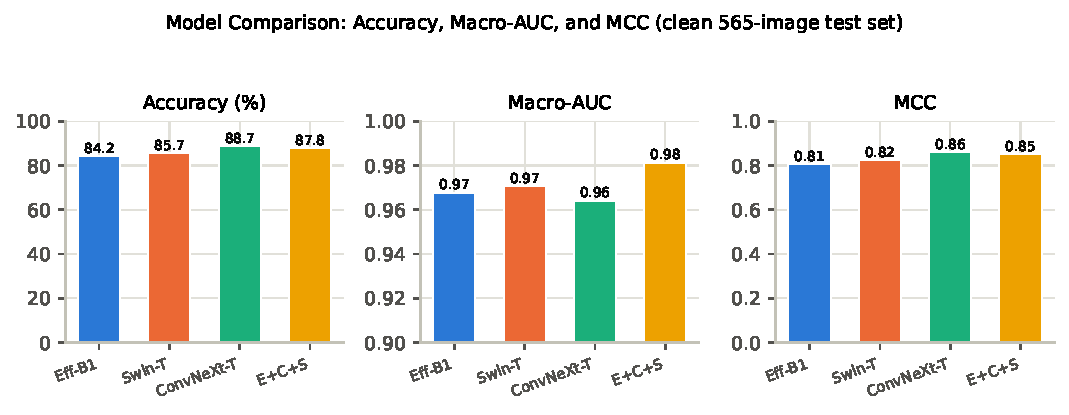
\includegraphics[width=\columnwidth]{Figure_3.pdf}
\caption{Model comparison: accuracy, macro-AUC, and MCC for each
backbone and the proposed ensemble (clean 565-image test set).}
\label{fig:comparison}
\end{figure}

\begin{figure}[!htbp]
\centering
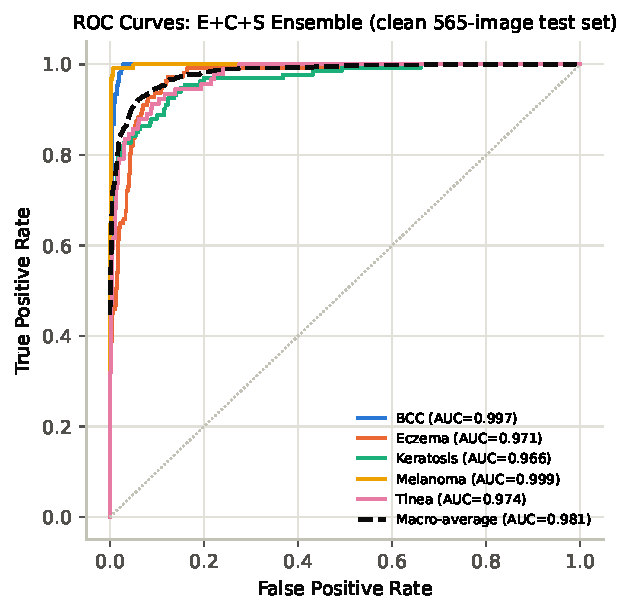
\includegraphics[width=\columnwidth]{Figure_4.pdf}
\caption{ROC curves for the proposed ensemble, per class and
macro-average (clean 565-image test set).}
\label{fig:roc}
\end{figure}

\begin{figure}[!htbp]
\centering
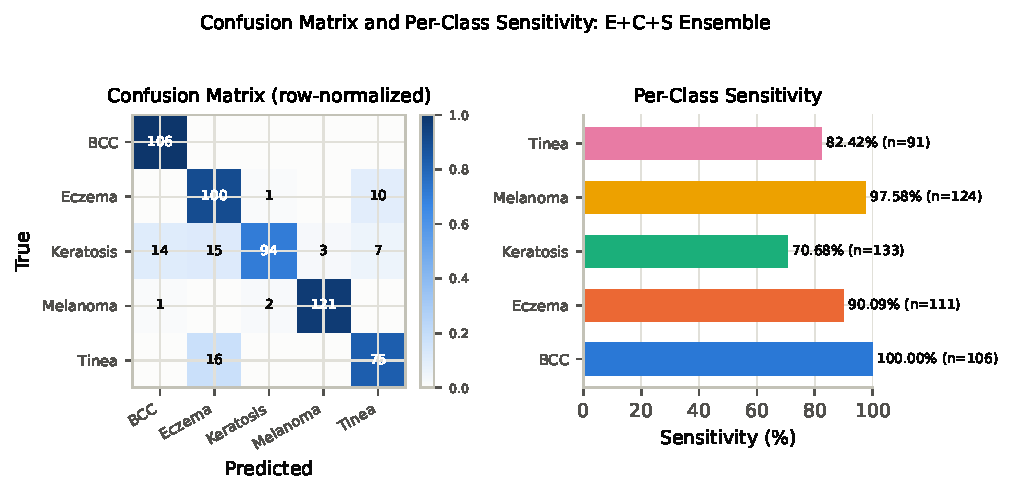
\includegraphics[width=\columnwidth]{Figure_5.pdf}
\caption{Confusion matrix (row-normalized) and per-class sensitivity for
the proposed ensemble.}
\label{fig:confusion}
\end{figure}

\begin{figure}[!htbp]
\centering
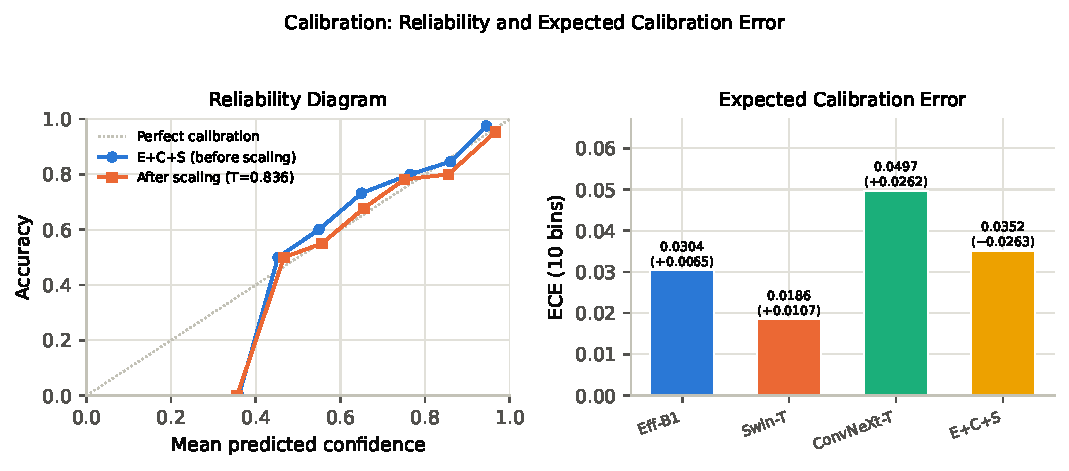
\includegraphics[width=\columnwidth]{Figure_6.pdf}
\caption{Calibration: reliability diagram before and after temperature
scaling, and Expected Calibration Error across configurations.}
\label{fig:calibration}
\end{figure}

% =======================================================================
\section{Discussion}\label{sec:discussion}
% =======================================================================

\subsection{Clinical Interpretation}

The ensemble's value in this setting lies less in raising peak accuracy
than in improving the ranking quality of the predicted class probabilities
and in producing better-calibrated confidence scores. Both properties
matter more than raw accuracy for a system intended to present a ranked
differential diagnosis for clinician review rather than a single label: a
higher macro-AUC means the correct class is more reliably ranked near the
top even when it is not the argmax, and calibrated, non-overconfident
probabilities are what make a confidence-based triage rule
(Section~\ref{sec:methods}) behave as intended rather than escalating or
dismissing cases on a number that does not track actual correctness. That
ConvNeXt-Tiny -- the single most accurate backbone -- is also the
worst-calibrated and most overconfident supports evaluating and selecting
ensembles on calibration as well as accuracy, rather than on accuracy
alone, as is typical in the ensemble literature we build on
\cite{ref12,ref13,ref14,ref15,ref16,ref17}.

The residual confusion between eczema and tinea (Section~\ref{sec:results})
is consistent with clinical experience rather than a model-specific
weakness: both conditions present as scaly, erythematous, or
hyperpigmented plaques, and in melanin-rich skin the erythema that would
ordinarily help distinguish an eczematous plaque is frequently masked,
leaving annular scaling as the dominant visual cue. In routine practice the
two are often separated by potassium hydroxide microscopy rather than
visual inspection alone, so a purely image-based classifier is being asked
to resolve a distinction that dermatologists themselves do not always
attempt on morphology alone. The keratosis-to-basal-cell-carcinoma
confusion mirrors a known clinical overlap between pigmented actinic
keratoses and superficial basal cell carcinomas, compounded here by
keratosis receiving no clinical loss boost during training
(Section~\ref{sec:methods}).

\subsection{Comparison with Prior Ensemble Work}

Heterogeneous ensembles combining convolutional and attention-based
backbones have been reported to outperform their individual members on
dermoscopic benchmarks \cite{ref12,ref13,ref14,ref15,ref16,ref17}, but
these evaluations are justified on accuracy and AUC alone and are
conducted on datasets drawn predominantly from lighter Fitzpatrick skin
types. Uncertainty and calibration have been studied for skin-lesion
classifiers elsewhere, for example with deep ensembles evaluated on the
dermoscopic HAM10000 corpus,
% VERIFY: LoRA-Ensemble citation and its calibration claim are not yet
% verified -- no bibliography entry exists for it yet (see
% Wiley-IJIST.md Phase 7 item 4).
but, to our knowledge, not for a heterogeneous convolutional-transformer
soft-voting ensemble on a melanin-rich clinical corpus. The present
study's contribution is therefore best read as extending this ensemble
literature along the calibration axis on a population it has not
previously been evaluated against, rather than as introducing a new fusion
mechanism: the decision-level averaging rule itself is standard and
deliberately simple (Section~\ref{sec:methods}).

\subsection{Limitations}

Several limitations bear directly on how these results should be read.
First, the three-backbone ensemble was selected as the proposed
configuration by comparison against the other six subsets on the same
held-out test set used to report its final performance
(Section~\ref{sec:results}); although the comparison that drives this
choice (ensemble vs.\ C+S on macro-AUC) is a statistically significant
one, no independent validation-based configuration search was performed,
so the selection and the reported performance are not fully separated.
Second, each backbone was trained once, with a single random seed, under a
training recipe that did not enable deterministic cuDNN operations; a
byte-identical retrain of one backbone reproduced its reported accuracy to
within 0.38 percentage points, which bounds but does not eliminate
seed-dependent variance in the reported numbers. Third, all results come
from a single corpus and a single train/validation/test partition; no
external validation on an independently collected dataset was performed,
and although the test set was de-duplicated against training and
validation images by perceptual hashing, the partition itself was
inherited rather than generated by an auditable, patient-aware procedure,
and no patient- or lesion-level identifiers are available across the five
aggregated sources to confirm that no patient contributes images to more
than one partition. Fourth, label provenance differs across the five
source datasets (a mix of biopsy-confirmed and clinical diagnoses) and is
not tracked per image in the assembled corpus, so a result is not
attributable to a single, consistent ground-truth standard. Fifth, and
most directly relevant to this study's stated population, consistent
skin-tone labels are not available across the five sources: the corpus was
assembled to emphasize melanin-rich presentations, but no Fitzpatrick
type, Monk Skin Tone, or individual typology angle label exists for most
images, so no tone-stratified performance claim is made or supported by
the present evaluation. Sixth, a preliminary individual typology angle
(ITA) analysis -- computed on the contaminated 727-image test set rather
than the de-duplicated 565-image set used for every other result in this
paper -- found a 12.01 percentage-point gap between the best-performing
(``intermediate,'' $n=93$, 94.62\%) and worst-performing (``brown,''
$n=92$, 82.61\%) tone bins, with non-overlapping 95\% bootstrap confidence
intervals; all three backbones showed the same qualitative ordering across
bins. This gap does not track ITA monotonically -- the worst-performing
bin is not the darkest category -- and the confound between tone bin and
disease-class composition has not been decomposed, so we report it as a
preliminary signal rather than a validated fairness result.

Two further lines of work build on the classification engine evaluated
here but are reported separately rather than in this paper: a Grad-CAM
faithfulness evaluation and a federated-learning feasibility study are
both in preparation as separate manuscripts and are not elaborated here.

% =======================================================================
\section{Conclusion}\label{sec:conclusion}
% =======================================================================

This study addresses skin disease classification in melanin-rich skin,
which remains underserved by diagnostic tools trained predominantly on
lighter Fitzpatrick skin types. We curated a five-class, 6,655-image
corpus from five public sources, audited it for cross-split near-duplicate
contamination, and evaluated all seven combinations of three independently
fine-tuned backbones -- EfficientNet-B1, Swin-Tiny, and ConvNeXt-Tiny -- on
a de-duplicated 565-image test set. The most accurate single backbone,
ConvNeXt-Tiny, was also the worst-calibrated and most overconfident. An
equal-weight three-backbone soft-voting ensemble achieved 87.79\% accuracy
and the highest macro-AUC (0.9813) of any configuration, including every
two-backbone subset, with the difference against the strongest
two-backbone alternative statistically significant on macro-AUC though not
on accuracy. The ensemble was also the only configuration with slightly
conservative rather than overconfident probabilities, and malignant-class
sensitivity remained high (100\% basal cell carcinoma, 97.58\% melanoma).
These results support selecting and reporting ensembles for dermatological
screening on calibration as well as accuracy, particularly where
confidence scores drive downstream clinical triage. The present evaluation
is limited to a single corpus, a single train/validation/test partition,
and populations for which consistent skin-tone labels are not available;
prospective and externally validated evaluation remains necessary before
clinical deployment.

% =======================================================================
% Mandatory statements -- Phase 8. Several fields below are placeholders
% explicitly marked VERIFY; the user must supply these before submission.
% =======================================================================

\bmsubsection*{Author Contributions}
% VERIFY: CRediT roles per author -- user to supply (14 standard roles;
% see Wiley-IJIST.md Phase 8).

\bmsubsection*{Acknowledgments}
% VERIFY: non-author help, compute resources, dataset creators -- user to
% supply.

\bmsubsection*{Financial Disclosure}
% VERIFY: matches \fundingInfo above -- user to supply, or state no
% specific grant was received.

\bmsubsection*{Ethics Statement}
This study used only publicly available, de-identified image datasets
(Fitzpatrick17k, PAD-UFES-20, DermaCon-IN, the Melanoma Cancer Image
Dataset, and the Skin Disease Image Dataset) released under their
respective licenses; no new data were collected from human participants.
% VERIFY: confirm this wording against each dataset's actual license and
% whether an institutional IRB exemption letter is required/available --
% see Wiley-IJIST.md Phase 8 and the checklist's suggested wording.

\bmsubsection*{Patient Consent Statement}
Not applicable: secondary analysis of publicly released, de-identified
datasets; consent was obtained by the original dataset creators where
required.

\bmsubsection*{Conflicts of Interest}
% VERIFY: the authors declare all conflicts of interest, or none -- user
% to confirm/supply.
The authors declare no conflicts of interest.

\bmsubsection*{Data Availability Statement}
% VERIFY: finalize per Wiley's template wording and the actual code/data
% release plan (GitHub release archived with a DOI, per the checklist).
These data were derived from the following resources available in the
public domain: Fitzpatrick17k, PAD-UFES-20, DermaCon-IN, the Melanoma
Cancer Image Dataset, and the Skin Disease Image Dataset. Split
manifests and code are available at [VERIFY: repository URL / DOI].

\bmsubsection*{AI Use Disclosure}
% VERIFY: user to confirm and supply the exact tool/version used, per
% Wiley's policy that substantive AI use must be described transparently.

% =======================================================================
% Bibliography -- inline thebibliography, numbered (VANCOUVER style
% option above), no bibtex run required. Only entries actually cited in
% this manuscript are listed; ref3/ref4/ref7/ref8/ref9/ref13/ref16-25 from
% the old main_updated.tex bibliography are NOT carried over since the
% Literature Review section (which cited them) was redistributed/cut in
% this version -- renumber if any of those return in a later revision.
% =======================================================================

\begin{thebibliography}{99}

\bibitem{ref1}
Aboulmira, A., Hrimech, H., Lachgar, M.: Skin diseases classification with machine learning
and deep learning techniques: A systematic review. International Journal of Advanced Computer
Science and Applications \textbf{15}(10), 1155--1173 (2024)
% VERIFY: Phase 7 found this citation does not support the clinical-outcomes
% claim it is near in the Introduction -- see inline VERIFY comment above.
% Kept in the bibliography pending a decision on whether to drop or
% repurpose it; currently it is NOT cited anywhere in the main text.

\bibitem{ref2}
Yan, S., Yu, Z., Primiero, C., Vico-Alonso, C., Wang, Z., Yang, L., Tschandl, P., Hu, M.,
Ju, L., et al.: A multimodal vision foundation model for clinical dermatology. Nature Medicine
\textbf{31}(8), 2691--2702 (2025)

\bibitem{ref3}
Ward, A., Li, J., Wang, J., Lakshminarasimhan, S., Carrick, A., Campana, B., Hartford, J.,
et al.: Creating an empirical dermatology dataset through crowdsourcing with web search
advertisements. JAMA Network Open \textbf{7}(11), e2446615 (2024)

\bibitem{ref4}
Gottfrois, P., Gr\"{o}ger, F., Andriambololoniaina, F.H., Amruthalingam, L.,
Gonzalez-Jimenez, A., Hsu, C., Kessy, A., Lionetti, S., et al.: PASSION for dermatology:
Bridging the diversity gap with pigmented skin images from Sub-Saharan Africa. In: Medical
Image Computing and Computer Assisted Intervention -- MICCAI 2024, Lecture Notes in Computer
Science, vol. 15003, pp. 703--712. Springer, Cham (2024)

\bibitem{ref5}
Madarkar, S.S., Madarkar, M., Madhumitha, V., Prakash, T., Mopuri, K.R., Vinaykumar, M.V.,
Sathwika, K.V.L., et al.: DermaCon-IN: A multi-concept annotated dermatological image dataset
of Indian skin disorders for clinical AI research. In: Advances in Neural Information
Processing Systems (NeurIPS), Datasets and Benchmarks Track (2025)

\bibitem{ref6}
Ben\v{c}evi\'{c}, M., Habijan, M., Gali\'{c}, I., Babin, D., Pi\v{z}urica, A.: Understanding
skin color bias in deep learning-based skin lesion segmentation. Computer Methods and Programs
in Biomedicine \textbf{245}, 108044 (2024)

\bibitem{ref10}
Housley, P.P., Samia, A.M., Motaparthi, K.: Performance evaluation of ChatGPT-4o in
dermatological diagnoses across Fitzpatrick skin types. Cureus (2025).
https://doi.org/10.7759/cureus.87368

\bibitem{ref11}
Ayas, S.: Multiclass skin lesion classification in dermoscopic images using Swin Transformer
model. Neural Computing and Applications \textbf{35}(9), 6713--6722 (2023)

\bibitem{ref12}
Hao, S., Zhang, L., Jiang, Y., Wang, J., Ji, Z., Zhao, L., Ganchev, I.: ConvNeXt-ST-AFF: A
novel skin disease classification model based on fusion of ConvNeXt and Swin Transformer.
IEEE Access \textbf{11}, 117460--117473 (2023)

\bibitem{ref13}
Liu, X., Wang, X., Liu, H., Zang, X., Li, L., Ji, Z., Ganchev, I.: FUSCANet: Enhancing skin
disease classification through feature fusion and spatial-channel attention mechanisms. IEEE
Access \textbf{13}, 100683--100698 (2025)

\bibitem{ref14}
Lilhore, U.K., Sharma, Y.K., Simaiya, S., Alroobaea, R., Baqasah, A.M., Alsafyani, M.,
Alhazmi, A.: SkinEHDLF: A hybrid deep learning approach for accurate skin cancer
classification in complex systems. Scientific Reports \textbf{15}, 14913 (2025)

\bibitem{ref15}
Thwin, S.M., Park, H.-S.: Skin lesion classification using a deep ensemble model. Applied
Sciences \textbf{14}(13), 5599 (2024)

\bibitem{ref16}
Thwin, S.M., Park, H.-S.: Enhanced skin lesion segmentation and classification through
ensemble models. Eng \textbf{5}(4), 2805--2820 (2024)

\bibitem{ref17}
Asif, S., Zhao, M., Li, Y., Tang, F., Zhu, Y.: CFI-Net: A Choquet fuzzy integral based
ensemble network with PSO-optimized fuzzy measures for diagnosing multiple skin diseases
including Mpox. IEEE Journal of Biomedical and Health Informatics \textbf{28}(9), 5573--5586
(2024)

\bibitem{ref26}
Loshchilov, I., Hutter, F.: Decoupled weight decay regularization. In: International Conference
on Learning Representations (ICLR) (2019)

\bibitem{ref27}
Hu, J., Shen, L., Sun, G.: Squeeze-and-excitation networks. In: Proceedings of the IEEE
Conference on Computer Vision and Pattern Recognition (CVPR), pp. 7132--7141 (2018)

% VERIFY: add entries for Fitzpatrick17k, PAD-UFES-20, the Melanoma Cancer
% Image Dataset, and SDID (see Wiley-IJIST.md Phase 7 \S2.2 for two
% drafted candidates and two still-unidentified sources), and for the
% LoRA-Ensemble paper cited in Discussion \S4.2 once verified.

\end{thebibliography}

\end{document}
